\section{Try It Out}\label{s:try-it}

All of the components discussed in this paper have been implemented as
units~\cite{local:flatt-pldi98} in Racket~\cite{dvanhorn:plt-tr1}.  We have
also implemented a ⸨#lang⸩ language so that composing and experimenting with
these interpreters is easy.  Assuming Racket is installed, you can install the
⸨monadic-eval⸩ package with (URL redacted for double-blind):
%\begin{center}
%\begin{verbatim}
%raco pkg install https://github.com/plum-umd/monadic-eval.git
%\end{verbatim}
%\end{center}

A ⸨#lang monadic-eval⸩ program starts with a list of
components, which are linked together, and an expression producing an
evaluator.  Subsequent forms are interpreted as expressions when run.
Programs can be run from the command-line or interactively in the
DrRacket IDE.  For example, Figure~\ref{f:screen} shows a screen shot of the PDCFA
evaluator running the example from Section~\ref{s:cache}.

\begin{figure}
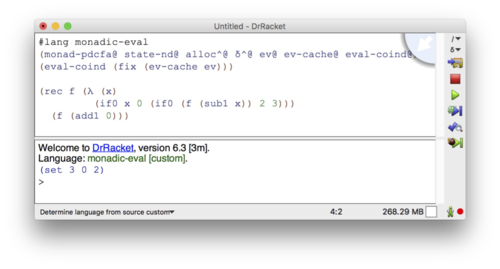
\includegraphics[width=\linewidth]{screen.png}
\caption{Screenshot of Monadic Language}
\label{f:screen}
\end{figure}
